\documentclass{article}


\usepackage{arxiv}

\usepackage[utf8]{inputenc} % allow utf-8 input
\usepackage[T1]{fontenc}    % use 8-bit T1 fonts
\usepackage{hyperref}       % hyperlinks
\usepackage{url}            % simple URL typesetting
\usepackage{booktabs}       % professional-quality tables
\usepackage{amsfonts}       % blackboard math symbols
\usepackage{nicefrac}       % compact symbols for 1/2, etc.
\usepackage{microtype}      % microtypography
\usepackage{lipsum}
\usepackage{multirow}
\usepackage{graphicx}


\title{Artist Identification	\\  A comparison between AlexNet, GoogLeNet and ResNeXt}


\author{
  Mattia Bottaro \\
  Dipartimento  di Matematica\\
  Università di Padova \\
  \texttt{mattia.bottaro@studenti.unipd.it} \\
  %% examples of more authors
   \And
  Mauro Carlin \\
Dipartimento  di Matematica\\
Università di Padova \\
\texttt{mauro.carlin@studenti.unipd.it} \\
  %% \AND
  %% Coauthor \\
  %% Affiliation \\
  %% Address \\
  %% \texttt{email} \\
  %% \And
  %% Coauthor \\
  %% Affiliation \\
  %% Address \\
  %% \texttt{email} \\
  %% \And
  %% Coauthor \\
  %% Affiliation \\
  %% Address \\
  %% \texttt{email} \\
}

\begin{document}
\maketitle

\begin{abstract}
	\textit{In this essay we present our work for the project of the Cognitive Services course.
	The problem we face is the artist identification, that is being able to recognize the author of a painting, given an image of it. Our dataset consists of about 10.000 paintings of 23 different artists.
	In order to resolve this task, we have exploited some famous Convolutional Neural Networks (CNNs), i.e. AlexNet, GoogLeNet and ResNeXt, that come with \textit{Pytorch} library. Those networks have been trained according to two distinct approaches: training them from scratch or exploiting pre-trained models using transfer learning technique. We used a virtual machine (VM) hosted by \textit{Google Cloud Platform} to perform our experiments.\\
	What we have achieved is a set of results which are in line or even better with the state-of-the-art, confirming that CNNs are suitable to solve this type of task.}
\end{abstract}


% keywords can be removed
\keywords{Convolutional Neural Network \and Artist Identification  \and ResNeXt \and GoogLeNet \and AlexNet \and Transfer Learning}


\section{Introduction}
Artist identification is the task of recognizing the author of a painting given only an image of it, without any other information about it. It's still nowadays a difficult problem to solve, for the following reasons:
\begin{itemize}
	\item there are not many contributions in the state-of-the-art, moreover the majority of them regards style identification and rely on old deep learning approaches;
	\item the available datasets are not as large as those used by models which solve more common tasks, such as image classification (e.g. Imagenet \cite{imagenet});
	\item artist's style could change a lot through his works, or it could be influenced by other painters. Therefore, it is clear how much is complicated to correctly classify a painting. 
\end{itemize}
Usually this task is done by human experts because of its difficulty, so our contribution can help to automatize the catalogation of artworks, which is more and more important due to the increasing number of  digital archives. In addition, our work could be useful in art forgeries detection.\\
Our approach involves 3 different CNNs, AlexNet (\cite{alexnet}), GoogLeNet (\cite{googlenet}) and ResNeXt (\cite{resneXt}), trained from scratch and with transfer learning in order to compare these opposite techniques. Our experiments yielded a top-1 accuracy of 82\%  and a top-3 accuracy of 94\% as best result.\\


The rest of the essay is structured as follows: in section \ref{relwor} we discuss  similarities and differences between previous works and ours. In section \ref{dataset} we explain the dataset we have used, how it was created and which preprocessing and data augmentation techniques we have exploited. In section\ref{method}
we discuss our approach for solving the problem we have just described. In \ref{experiments} we show some details regarding the \textit{GCloud Compute Engine}'s configuration, the metrics used to evaluate the goodness of the models and the detailed results of our experiments. Finally, in section \ref{conclusions} we draw some conclusion and we outline some possibile future works which rely on our result.


\section{Related Works}\label{relwor}

In this section we show some previous works related to ours. In addition to define the references of our experiments, the following should further convince the reader of present-day difficulty in achieving good precision in artist identification.\\
Recently CNNs have become widespread, because of the good performance and results obtained in tasks regarding visual recognition.
Previous works not regarding CNNs use some famous approaches of features detection, such as Scale Invariant Feature Transforms (SIFT) and Histograms of oriented gradients (HOG) (\cite{Saleh2015}, \cite{mensink2014}, \cite{lombardi05}, \cite{jou2011}), to extract some particular characteristics of the painting useful for its classification. These works have in common the use of an SVM 1-vs-rest classifier, except \cite{jou2011} which uses both SVM 1-vs-rest and Naïve Bayes classifier. However, \cite{lombardi05} and \cite{jou2011} face up the problem of style recognition, which is different than artist identification, but using similar approaches.\\
In addition, some of these perform on small or not so heterogenous datasets, such as \cite{mensink2014} which uses the artworks of a single museum, or \cite{jou2011} which focuses on only 5 artists. Instead, in our work we set our sights on recognizing 23 different artists, with 450 paintings for each of them as our dataset. \\
In any case, these techniques are known to be not so effective due to the fact that features characterizing an artist's style can be many and difficult to engineer, such as texture, shape, color, tone, variety, proportion, pattern and brush strokes.\\

One of the results achieved in \cite{hong2017} shows an improvement of performance using CNNs up to 13.6 percentage points more than SIFT, HOG or similar.  This work aims to detect artwork that violates copyright terms in television programs, TV series, movies or similar scenarios. They use different techniques to distort the images on their dataset in order to simulate potential situation that it would be appeared on TV programs or photographs or
movies. This is not suitable for our context because distortion would be harmful for artist identification.\\
They have experimented 3 different CNNs inspired by AlexNet and VGG, training them from scratch with a weights initialization according to a Gaussian distribution, instead, in our work, we use pre-existing CNNs without modifying their architectures. \cite{hong2017} is one of the few works which does not use SVM as classifier, but 3 fully connected layers with softmax classifier.\\
\textbf{Other works like \cite{Bar2014} and \cite{razavian2014} use} a CNN to generate features, then use an SVM 1-vs-rest classifier on top of it.
\cite{ArtistIdCNN406} exploit one of the most recent CNNs, i.e. ResNet (\cite{resnet}). It is an ancestor of ResNeXt (\cite{resneXt}), one of the CNNs used in our experiment. In \cite{ArtistIdCNN406} either training from scratch and training through transfer learning are studied,  as in our work.
\\

In the latest years, the number of CNNs for visual recognition is growing, as well as their contributions in the field of computer vision. Instead of hand-crafting features, CNNs are able to learn features representation of an image, making easier and more accurate this kind of task. What is missing is a performance comparison between the latter models in the field of artist identification and, more generally, in art-recognition tasks. This comparison is the purpose of our work.


\section{Dataset}\label{dataset}
\subsection{Overview}\mbox{}\\
The first requirement to train a CNN for artist identification is a dataset, concerning paintings of different artist, as large as possible. For our project we obtain a dataset from \cite{ArtGANDataset}, which is a subset of the WikiArt Dataset. \\
The dataset contains about 19,000 images of 23 different artists, regarding very different styles, genres  and epochs. There are also 3 \textit{.csv} files that labelled all the paintings for genre, style, and artist: for our work we have used only the last one. In order to obtain a balanced dataset, we decided to randomly select 450 paintings for each artist, so in the end our dataset contains of 10,350 total images. \\
The next step was to divided the entire dataset in training, validation and test sets. \cite{ArtGANDataset} suggests a possibile partitioning, but we decided to create our own because they did not provide a test set, and some paintings included in the training set are also in the validation set, fact that could create a distorted evaluation of our model during training. Therefore, we split the dataset in training, validation and test sets using a 80-10-10 division per artist, obtaining a training set of 360 paintings per artist, and a validation and test sets each of 45 paintings per artist.

\subsection{Preprocessing and Data augmentation}\mbox{}\\
CNNs require a precise size for their input images, so we had to modify the paintings in the dataset, considering that they vary widely in shape and size.\\
So, first, we take a 224$\times$224 crop of each input images, next we zero-center and normalize them, with mean and standard deviation calculated for each of the three channels red, green and blue (they are RGB images).  \\
During training we also randomly horizontally flip the image with a probability of 50\%, and also take a random crop of it (not always the central pixels), for essentialy two reasons:
\begin{itemize}
	\item randomness create variety and can avoid overfit;
	\item we assumed that the style of an artist is present everywhere in the painting, so taking random crops do not influence the performance of our models.
\end{itemize}
Instead, for validation and test sets we always have taken a central crop, in order to obtain stable results comparable between different epochs.

\section{Method}\label{method}
In our work we have considered three different CNNs: AlexNet, GoogLeNet and ResNeXt. Every network takes as input a
3$\times$224$\times$224 RGB image and outputs the scores for each of the 23 artists present in our dataset.
\\
For all of our networks, we use a softmax classifier with
cross-entropy loss:
\begin{equation}
L_{i}=-\log \left(\frac{e^{f_{y_{i}}}}{\sum_{j} e^{f_{j}}}\right)
\end{equation}
\textbf{SPIEGARE}

First, we have trained the networks from scratch, in order to allow them to learn features solely for artist identification. \\
Afterwards, starting from networks with weights pre-trained on ImageNet dataset, we trained them using transfer learning to understand if a features representation from ImageNet is a valuable starting point for our problem.\\
In both approaches, we replaced the last fully-connected layer of the CNNs with a new one to calculate a score for each artist in
our dataset. We used \cite{pytorchguide} as a guide for replacing the fully-connected layer, and for performing transfer learning on the pre-trained networks.

\subsection{AlexNet}
AlexNet (\cite{alexnet}) was the winning entry in ILSVRC 2012. It solves the problem of image classification where the input is an image of one of 1000 different classes (e.g. cats, dogs etc.) and the output is a vector of 1000 numbers, achieving a top-5 error of 15.8\%.
Architecture (Figure \ref{fig:alexnet}) is made up of 8 layers, 5 convolutional, some of them followed by max pooling layers, and 3 fully-connected, with ReLU as activation function.\\
AlexNet also uses dropout (\cite{dropout}) to reduce overfitting. In this strategy, a neuron is dropped from the network with a probability of 50\%. When a neuron is dropped, it does not contribute to either forward or backward propagation. 
As a result, the learnt weight parameters are more robust and do not get overfitted easily.\\
We decided to include AlexNet in our work because it represent the most important starting point of image classification with CNN, so it would be interesting to compare its performance on our task with more recent, complex and deep networks.

\begin{figure}[h]
	\centering
	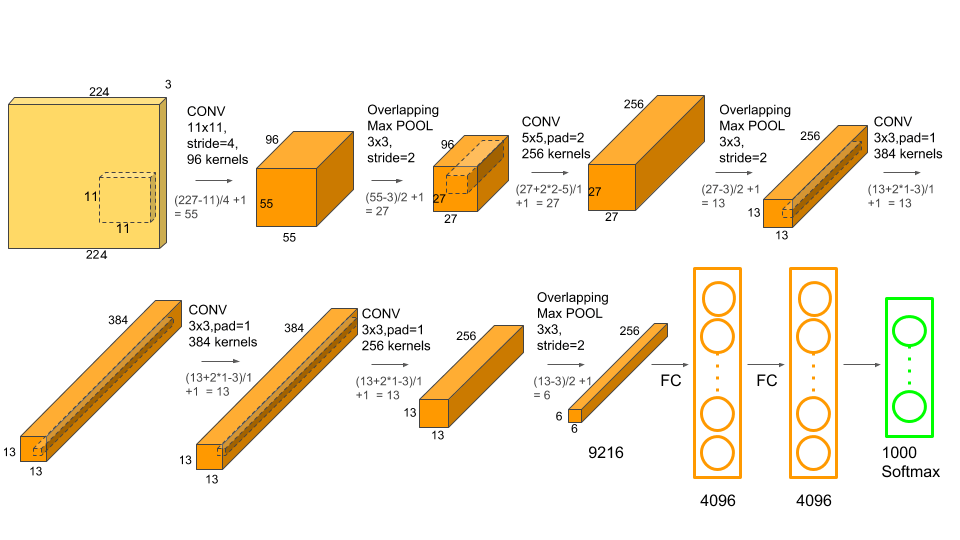
\includegraphics[width=0.7\linewidth]{image/AlexNet}
	\caption{AlexNet's architecture}
	\label{fig:alexnet}
\end{figure}

\subsection{GoogLeNet}
GoogLeNet (\cite{googlenet}) won the ILSVRC 2014 achieving 6.67\% top-5 error on ImageNet. We considered this netowrk in our work PERCHè HA OTTENUTO IMPROVMENT NOTEVOLE DALL'ANNO PRECEDENTE, QUINDI INTRODUCENDO INNOVAZIONE CHE EFFETTI AMENTE FUNZONAO.
It is composed of 22 layers, with different innovations regarding the fully-connected layers, the vanishing gradient problem and a new inception module.\\
An interesting addition to the architecture is to change the second last fully-connected layer with an average pooling layer. This layer spatially averages the feature map, converting 7x7x1024 input to 1x1x1024, reducing the computation and the number of parameters, by a factor of 49. This average pooling layer is finally followed by a normal fully-connected layer with 1000 neurons (and 1024x1000 parameters), for the 1000 ImageNet classes.
During training, to address the vanishing gradient problem, special extra structures are added to the network (these are removed during testing). These are auxiliary classifiers attached to intermediate layers. All the losses from each classifier gets added up, taking contribution from the auxiliary classifier lower
than the main one, during training. The gradient from the main classifier which would have otherwise become very small, and thus slowing training, by time it reached the lower initial layers, receives gradient from the auxiliary classifiers and thus the net gradient becomes big enough to allow training to progress.
\begin{figure}[h]
	\centering
	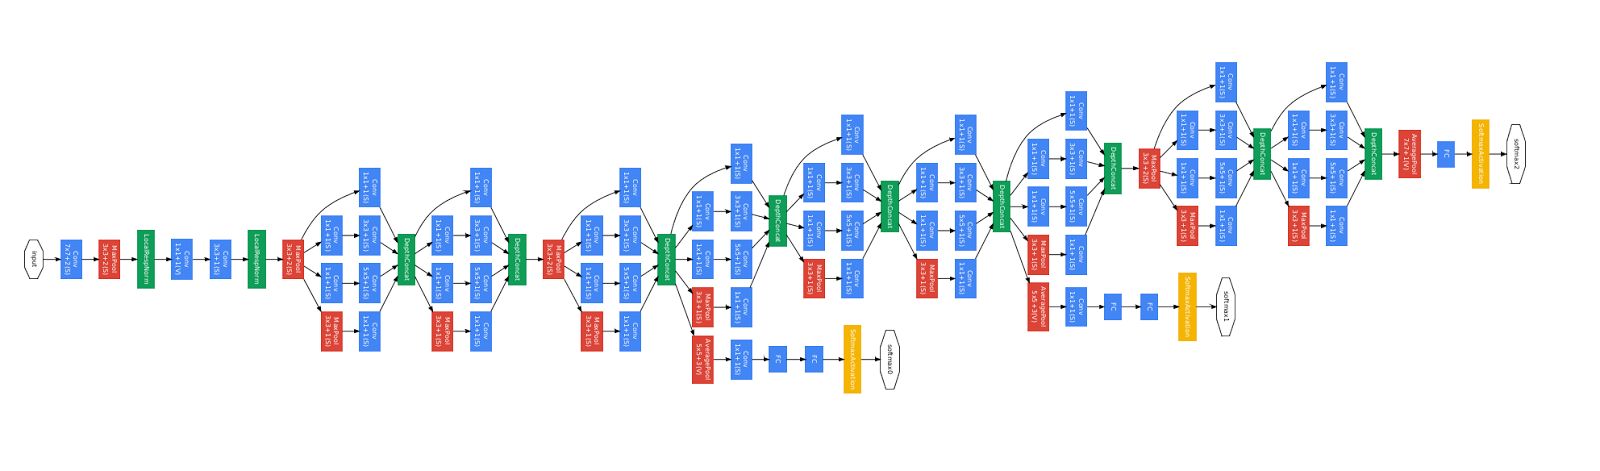
\includegraphics[width=0.7\linewidth]{image/GoogLeNet}
	\caption[]{GoogLeNet's architecture}
	\label{fig:googlenet}
\end{figure}

\subparagraph{Inception module}\mbox{}\\
The Inception modules were designed to solve the problem of computational expense, as well as overfitting, among other issues. The solution, in short, is to take multiple filter sizes within the CNN, and rather than stacking them sequentially, ordering them to operate on the same level. \\
 The most simplified version of an inception module works by performing a convolution on an input with not one, but three different sizes of filters (1x1, 3x3, 5x5). Also, max pooling is performed. Then, the resulting outputs are concatenated and sent to the next layer.
A method to reduce the number of computation is dimensionality reduction. This involves convolutions with 1x1 filters before convolutions with bigger filters (figure \ref{fig:incmodule}).
\begin{figure}[h]
	\centering
	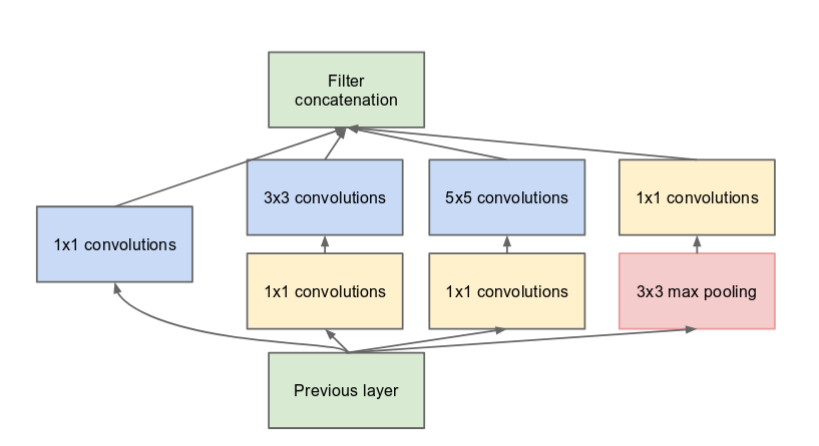
\includegraphics[width=0.7\linewidth]{image/inc_module}
	\caption{Inception module with dimension reduction}
	\label{fig:incmodule}
\end{figure}




\subparagraph{ResNeXt}
ResNeXt (\cite{resneXt})was the first runner up in ILSVRC 2016, achieving 3.03\% top-5 error rate, which is a better result than human precision on the same dataset (5.1\% error). The model's name, ResNeXt, contains Next. It means the next dimension, on top of the ResNet, namely the winner in ILSVRC 2015. This next dimension is called the “cardinality” dimension.\\
The architecture adopts VGG/ResNets' strategy of repeating layers, while
exploiting the split-transform-merge strategy (for example inception modules have the same approch, that is, input is split into a few lower-dimensional embeddings, transformed by a set of specialized filters, and merged by concatenation). 
A module in this network performs a set of transformations, each on a low-dimensional embedding, whose outputs are aggregated by summation. The transformations to be aggregated are all of the same topology (Figure \ref{fig:resnext_block} (right)).\\

\begin{figure}[h]
	\centering
	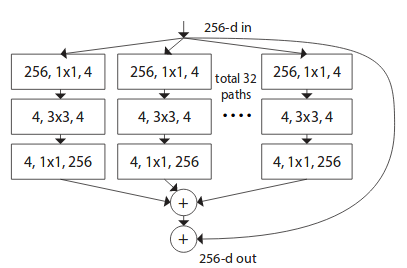
\includegraphics[width=0.7\linewidth]{image/resnext}
	\caption{Left: A block of ResNet. Right: A block of ResNeXt with cardinality=32. A layer is shown as (\# in channels, filter size, \# out channels)}
	\label{fig:resnext_block}
\end{figure}

Experiments in \cite{resneXt} demonstrate that increasing cardinality (the size of the set of transformations) is a more effective way of gaining accuracy than going deeper or wider, especially when depth and width starts to give diminishing returns for existing models.\\
In our work we use ResNeXt-50 32$\times$4d (Figure \ref{fig:res}), that represents a network with four bottleneck, and each layer having cardinality of 32. 

\begin{figure}
	\centering
	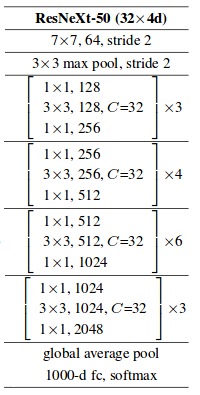
\includegraphics[height=0.4\linewidth]{image/res}
	\caption{ResNeXt-50 (32$\times$4)'s architecture}
	\label{fig:res}
\end{figure}
\section{Experiments}\label{experiments}

\subsection{Setup}
Both the built models and the experiments have been implemented in Pytorch (\cite{pytorch}). The reason why we chose this library is because of the presence of models, pre-trained and not, that we wanted to study.\\
The training of the models and the experiments were performed on a virtual machine hosted by \textit{Compute Engine}, one of the services provided by Google Cloud Platform (\cite{gcloud}). Its configuration, shown in table \ref{table:specVM}, is a pre-setting provided by the service itself and designed for deep learning applications  (\cite{vmconfig}). The dataset was stored in a \textit{Google Cloud Storage}'s bucket, another service provided by Google Cloud Platform.

\begin{table}
	\centering
	\begin{tabular}{|l|l|} 
		\hline
		\textbf{Component} & \textbf{Specification}  \\ 
		\hline
		OS                 & Debian 9                \\
		vCPU               & 2                       \\
		RAM                & 13GB                    \\
		GPU                & 1X NVIDIA Tesla K80     \\
		Disk               & 100GB                   \\
		Disk Type          & SSD                     \\
		Availability Zone  & us-west1-b              \\
		\hline
	\end{tabular}
\\
\caption{VM specifications}
   	\label{table:specVM}
\end{table}

\subsection{Implementation Details}\label{ImplDet}

For each CNN, we tested their performance with different learning rate values ($10^{-2}, 10^{-3}, 10^{-4}, 10^{-5}$). We have observed that $10^{-3}$ is the value which allows to converge faster to the best results, thus all experiments we have performed use this learning rate.\\
In figure \ref{fig:lr} we report ResNeXt's performance based on these different values, where it's clear that the lowest value of learning rate slows down the training phase, instead higher values ($10^{-2}$) bring more instability in the accuracy trend.

\begin{figure}[h]
	\centering
	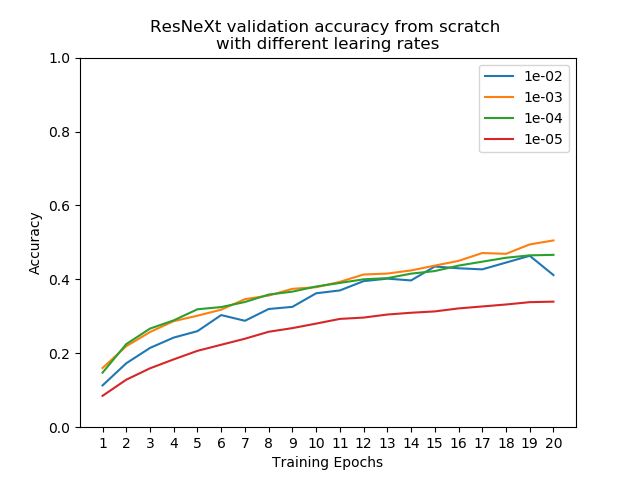
\includegraphics[width=.5\textwidth]{graphs/lr_scratch}\hfill
	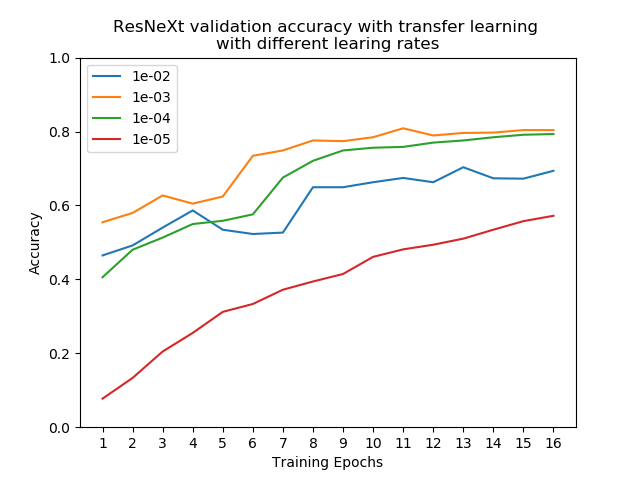
\includegraphics[width=.5\textwidth]{graphs/lr_tl}
	\caption{Top-1 accuracies for ResNeXt's validation set}
	\label{fig:lr}
\end{figure}

\textbf{We chose the Adam's update rule because the experiments using SGD were worse. \textbf{Abbiamo impostato il }learning rate $= 10^{-3}$ mentre per gli altri papametri we used the default ones, i.e. $\beta_{1}  = 0.9$ and $\beta_{2} = 0.999$.  \textbf{MA COSA SONO beta1 e BETA2}}\\

In transfer learning training, we set respectively the number of epochs and batch size to 16 and 32.  For each model chosen, pytorch makes available their final weights  trained on the ImageNet dataset (\cite{imagenet}), which makes transfer learning very easy to implement.\\
We first start training the network updating the weights only in the FC-layers, but the results obtained were not satisfactory.\\
With the aim of achieving higher accuracy, as experimented in \cite{ArtistIdCNN406}, we have decided to allow the update of the weights in the whole network when, for 3 consecutive epochs, the validation set's accuracy does not improve by 3 percentage points. When this condition occurs, learning rate is decreased by a factor of 10. This strong decrease is motivated by the hypothesis  that pre-trained weights are already "close" to those we are looking for, so it is good to update them with a smaller step-size.

In training from scratch, the number of epochs is set to 20, while the batch size is still 32.\\ 
Initialisation of the weights follows a uniform distribution in $[-x, x]$ where $x=1/\sqrt n$ and $n$ is the number of inputs to a given neuron (\textbf{STA COSA È DA VERIFICARE})\\
We have experimented what in pytorch is called \textit{scheduler}, i.e. every 7 epochs the learning rate is decreased by a factor of 10 . This strategy, however, has not led to improvements and in fact the results exposed have been obtained without the use of this technique.

In order to evaluate all the models that we study, we have calculated the accuracy on training and validation sets for each epochs during training, and the final accuracy on test set using the best weights resulted from training. The accuracy is intended as top-1, i.e.  the fraction of paintings whose artists are identify correctly, and top-3, i.e. the fraction of paintings whose artists are included in the 3 to whom the model has assigned the highest score.

\subsection{Results}\label{results}

In table \ref{table} we report the overall results obtained with training  from scratch and transfer learning for each CNN, including also the results obtained in \cite{ArtistIdCNN406}, \cite{Saleh2015} and \cite{mensink2014}, \textbf{OTHER}

The first thing we observe, comparing the CNNs, is that AlexNet's performances are much worse than other CNNs for all experiments, thus we can deduce how network's complexity allows to achieve better results. In fact, GoogLeNet and ResNeXt are successors of AlexNet, so this outcome should not be surprising. 
In particular, in training from scratch, AlexNet is 20 percentage points worse than others CNNs, while in training with transfer learning this distance is halved. This result shows that transfer learning performs very well in order to achieve quite good accuracy, even with not so complex networks. Indeed, AlexNet has obtained 87\% of top-3 accuracy in the test set.

For all the networks, we can see how training with transfer learning achieved results with 40 percentage points more than training from scratch. So, we can figure out that CNNs already trained on ImageNet dataset, which is wider than ours,  are a valuable starting point for artist identification\\
The most performing CNN is ResNeXt trained with transfer learning. Its top-1 accuracy reaches 82\% on test set, while its top-3 accuracy is roughly 94\%. This mean that it can narrow down the artist to three in the vast majority of cases.

Figure \ref{fig:confusion} shows the confusion matrix concerning our best network's classification on test set. Each row represents the true artist and each column represents the predicted one. Ideally, we want as many predictions as possible to be concentrated on the diagonal as this means that the network correctly predicted the true artist. The maximum possible value for a cell in the confusion matrix is 45, since there are 45 paintings per artist in the test set.\\
In general, we can easily see how the majority of artifacts are well-classified thanks to the colours (from yellow to brown) on the diagonal cell, i.e. more than 30 painting for each artist are well classified.

In particular, the artits better classified (44 out of 45) are Eugene Bodin, Ivan Aivazovsky and Raphael Kirchner. In fact, even though these artists may belong to differents artistic movements and styles, their painting tends to represent the world very close to reality (\textbf{figura ?? show some example}).\\
For example, Ivan Aivazovsky produced many portraits and landscapes, over half of all of his paintings are realistic depictions of coastal scenes and seascapes. The manner of painting real scenario or objects makes artist classification very similar to image classification. Indeed, from our results we note that artists with this characteristic obtained an higher accuracy.

For the artists whose paintings are often misclassified, we have noticed some common traits which follows.\\
Some of them belong to movements such as surrealism, cubism or expressionism, thus their artefacts are not depicting real scenario (\textbf{esempi}), making them harder to classify.
For example, Pablo Picasso, who founded the cubism movement, is the most misclassified artist (30 correctly classified out of 45).\\
The second reason leading to misclassification is the similarity  between different artists. The most striking example regards Ilya Repin, in fact, as we can see in Figure \ref{fig:confusion} (9th row, 2nd column), the model has classified Boris Kustodiev as authors of 8 Repin's artworks. This is not so surprising since Repin was the Kustodiev's teacher, influencing significantly his style. \\
Another reason concerns artists that, during their life, changed their art style significantly, producing very various type of paintings. For example in figure \ref{fig:vangogh} we can see 2 very different Van Gogh's artworks. This complicates furthermore the classification, leading to worse performance (accuracy on Van Gogh is 33 out of 45).

In figure \ref{fig:accscratch}, for each CNN trained from scratch,  we report the top-1 accuracy trends on training and validation set. What we can notice is that both trends are very close each other, proving a very low level of overfitting.
From this fact, we deduced that with a wider dataset and an higher number of epochs, we could obtained better performances. Therefore, we have decided to test once our best network for 30 epochs. We didn't extend this kind of experiment to all networks due to our limited Google Cloud's resources. As we expected, ResNeXt's accuracy trend \textbf{kept increasing} without introducing overfitting, improving both accuracies by 8 percentage points on test set.

In figure \ref{fig:acctransfer}, instead, we see the trends for each CNN trained with transfer learning. In all of them, after few epochs, an increase in the trend's slope is noted. This corresponds to the moment when the network is allowed to update not only the FC-layers' weights, but also those of all layers as previous explained in \ref{ImplDet}, adapting the whole CNN to artist identification task.\\
Moreover, we can see that GoogLeNet and ResNeXt, aftew roughly 10 epochs, are affected by overfitting. In fact there is an incresing difference between training accuracy and validation accuracy due to the stabilization of the latter, stating that these networks could have been trained for fewer epochs.  However, our results achieved higher accuracies than \cite{ArtistIdCNN406}, \cite{Saleh2015} and \cite{mensink2014}, \textbf{OTHER}


% Please add the following required packages to your document preamble:

\begin{table}[]
	\begin{tabular}{|c|c|c|c|c|}
		\hline
		\multicolumn{5}{|c|}{\textbf{Training from scratch}}                                                          \\ \hline
		\multirow{2}{*}{\textbf{Network}} & \multicolumn{2}{c|}{\textbf{Top-1}} & \multicolumn{2}{c|}{\textbf{Top-3}} \\ \cline{2-5} 
		& Train acc        & Test acc         & Train acc        & Test acc         \\ \hline
		AlexNet                           & 0.23103          & 0.27439          & 0.46159          & 0.51304          \\ \hline
		GoogLeNet                         & 0.42669          & 0.46956          & 0.68285          & 0.70628          \\ \hline
		ResNeXt-50                        & \textbf{0.50531} & \textbf{0.50048} & \textbf{0.74275} & \textbf{0.74782} \\ \hline
		ResNet-18 \cite{ArtistIdCNN406}                    & 0.516            & 0.511            & 0.737            & 0,710            \\ \hline
		1-vs-all SVM \cite{Saleh2015}                    & -            & 0.5776            &    -         & -            \\ \hline
		1-vs-all SVM (on 374 artist) \cite{mensink2014}                  & -            & 0.591            &    -         & -            \\ \hline
	\end{tabular}
	\begin{tabular}{|c|c|c|c|c|}
		\hline
		\multicolumn{5}{|c|}{\textbf{Training with transfer learning}}                                                           \\ \hline
		\multirow{2}{*}{\textbf{Network}} & \multicolumn{2}{c|}{\textbf{Top-1}}  & \multicolumn{2}{c|}{\textbf{Top-3}} \\ \cline{2-5} 
		& Train acc        & Test acc          & Train acc         & Test acc        \\ \hline
		AlexNet                           & 0.7134           & 0.68695           & 0.88925           & 0.87439         \\ \hline
		GoogLeNet                         & 0.87536          & 0.80579           & 0.96787           & 0.92492         \\ \hline
		ResNeXt-50                        & \textbf{0.92125} & \textbf{0.82318} & \textbf{0.98695}  & \textbf{0.94879} \\ \hline
		ResNet-18 \cite{ArtistIdCNN406}                    & 0.907            & 0.777             & 0.973             & 0.898           \\ \hline
	\end{tabular}
	\label{table}
\end{table}


\begin{figure}[htp]
	
	\centering
	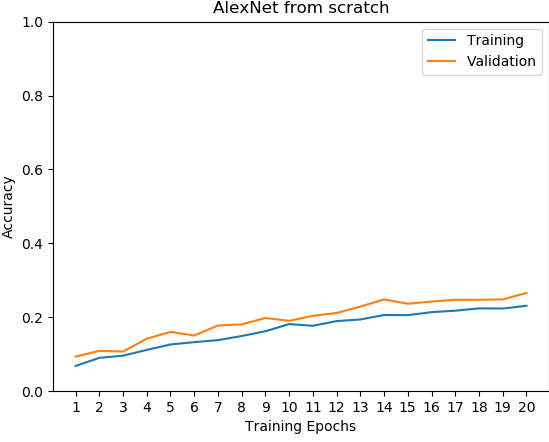
\includegraphics[width=.33\textwidth]{graphs/alex_scratch}\hfill
	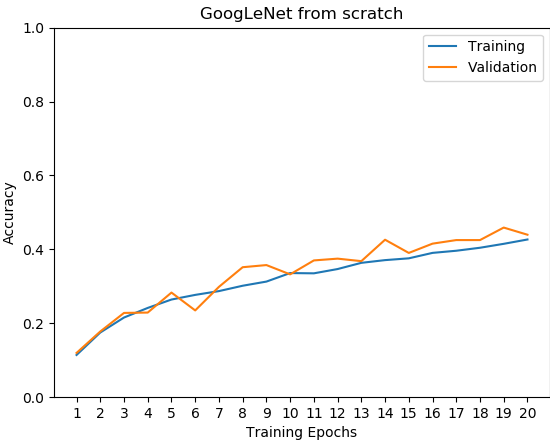
\includegraphics[width=.33\textwidth]{graphs/google_scratch}\hfill
	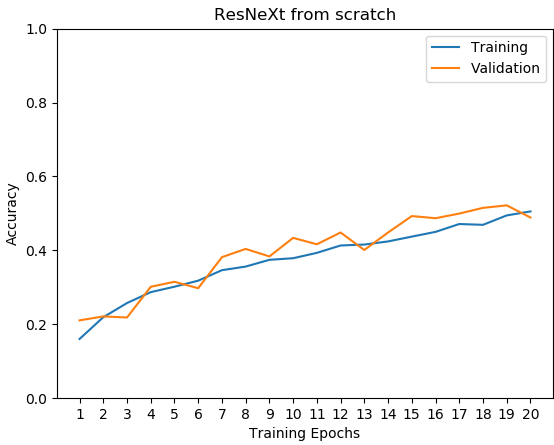
\includegraphics[width=.33\textwidth]{graphs/res_scratch}
	
	\caption{default}
	\label{fig:accscratch}
	
\end{figure}

\begin{figure}[htp]
	
	\centering
	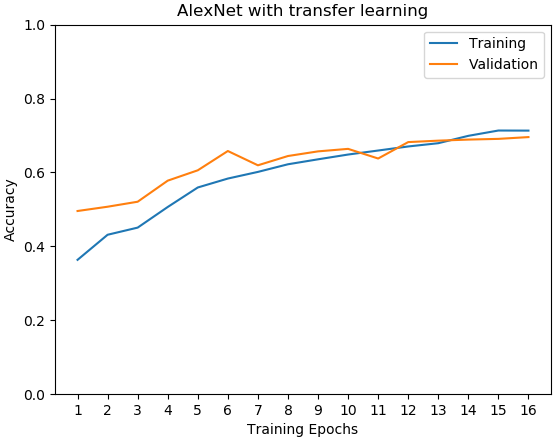
\includegraphics[width=.33\textwidth]{graphs/alex_training}\hfill
	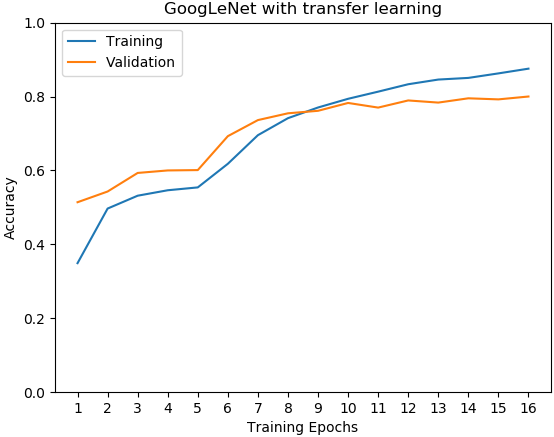
\includegraphics[width=.33\textwidth]{graphs/google_training}\hfill
	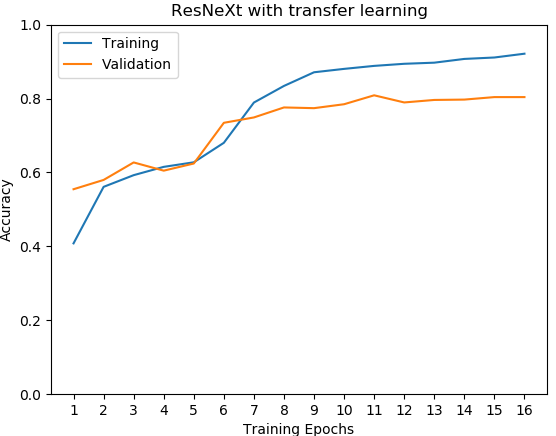
\includegraphics[width=.33\textwidth]{graphs/res_training}
	
	\caption{default}
	\label{fig:acctransfer}
	
\end{figure}

\begin{figure}
	\centering
	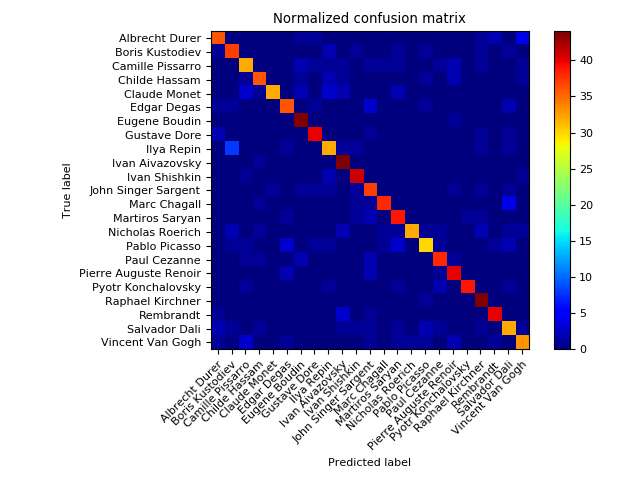
\includegraphics[width=0.8\linewidth]{graphs/confusion}
	\caption{Confusion matrix for top-1 classification on ResNeXt test set}
	\label{fig:confusion}
\end{figure}


\begin{figure}[htp]
	
	\centering
	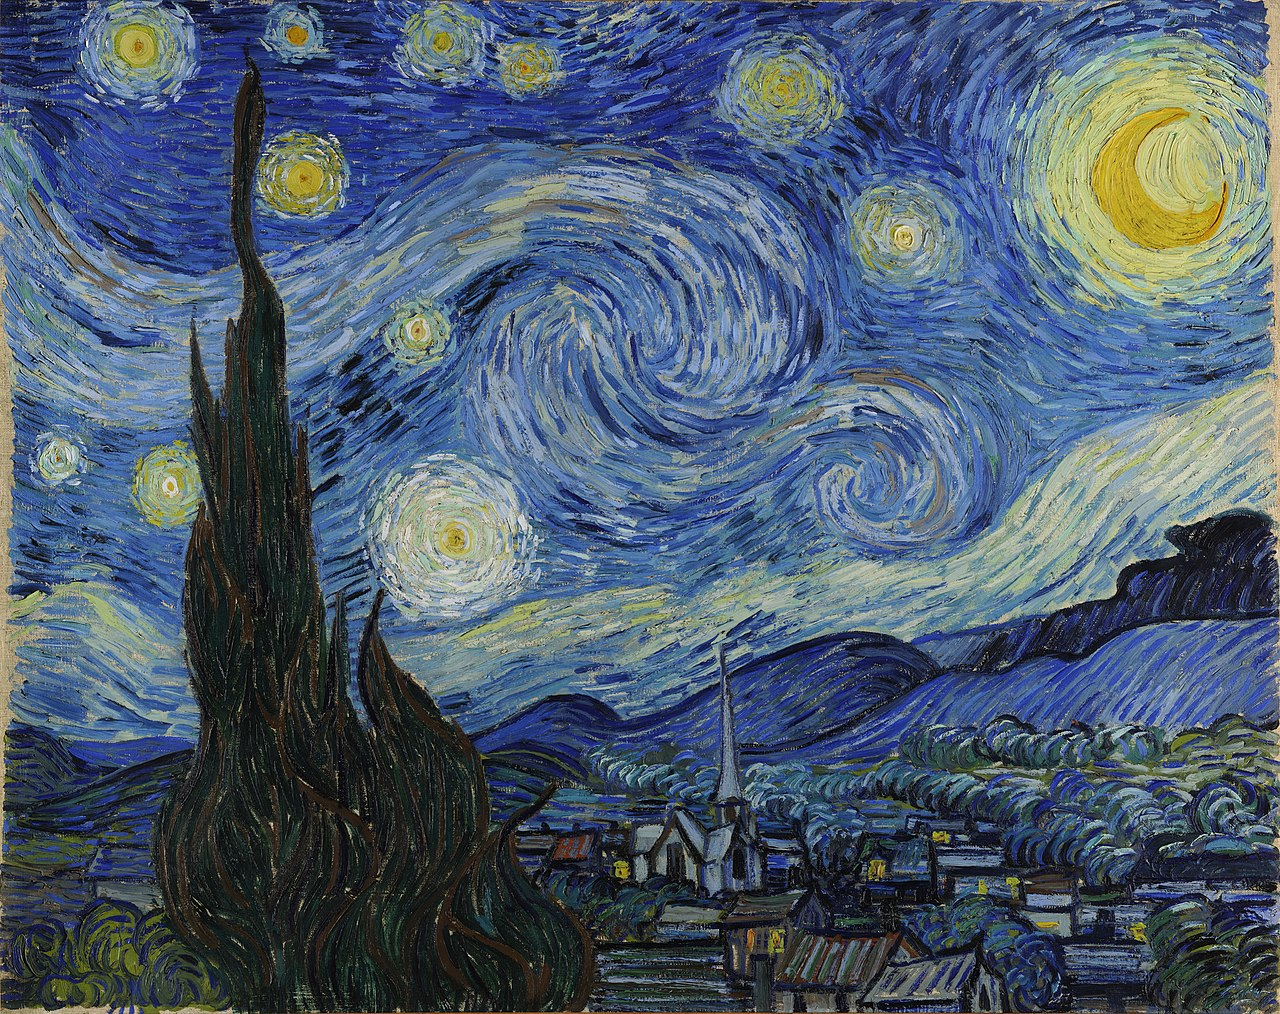
\includegraphics[width=.5\textwidth]{image/1280px-Van_Gogh_-_Starry_Night_-_Google_Art_Project}\hfill
	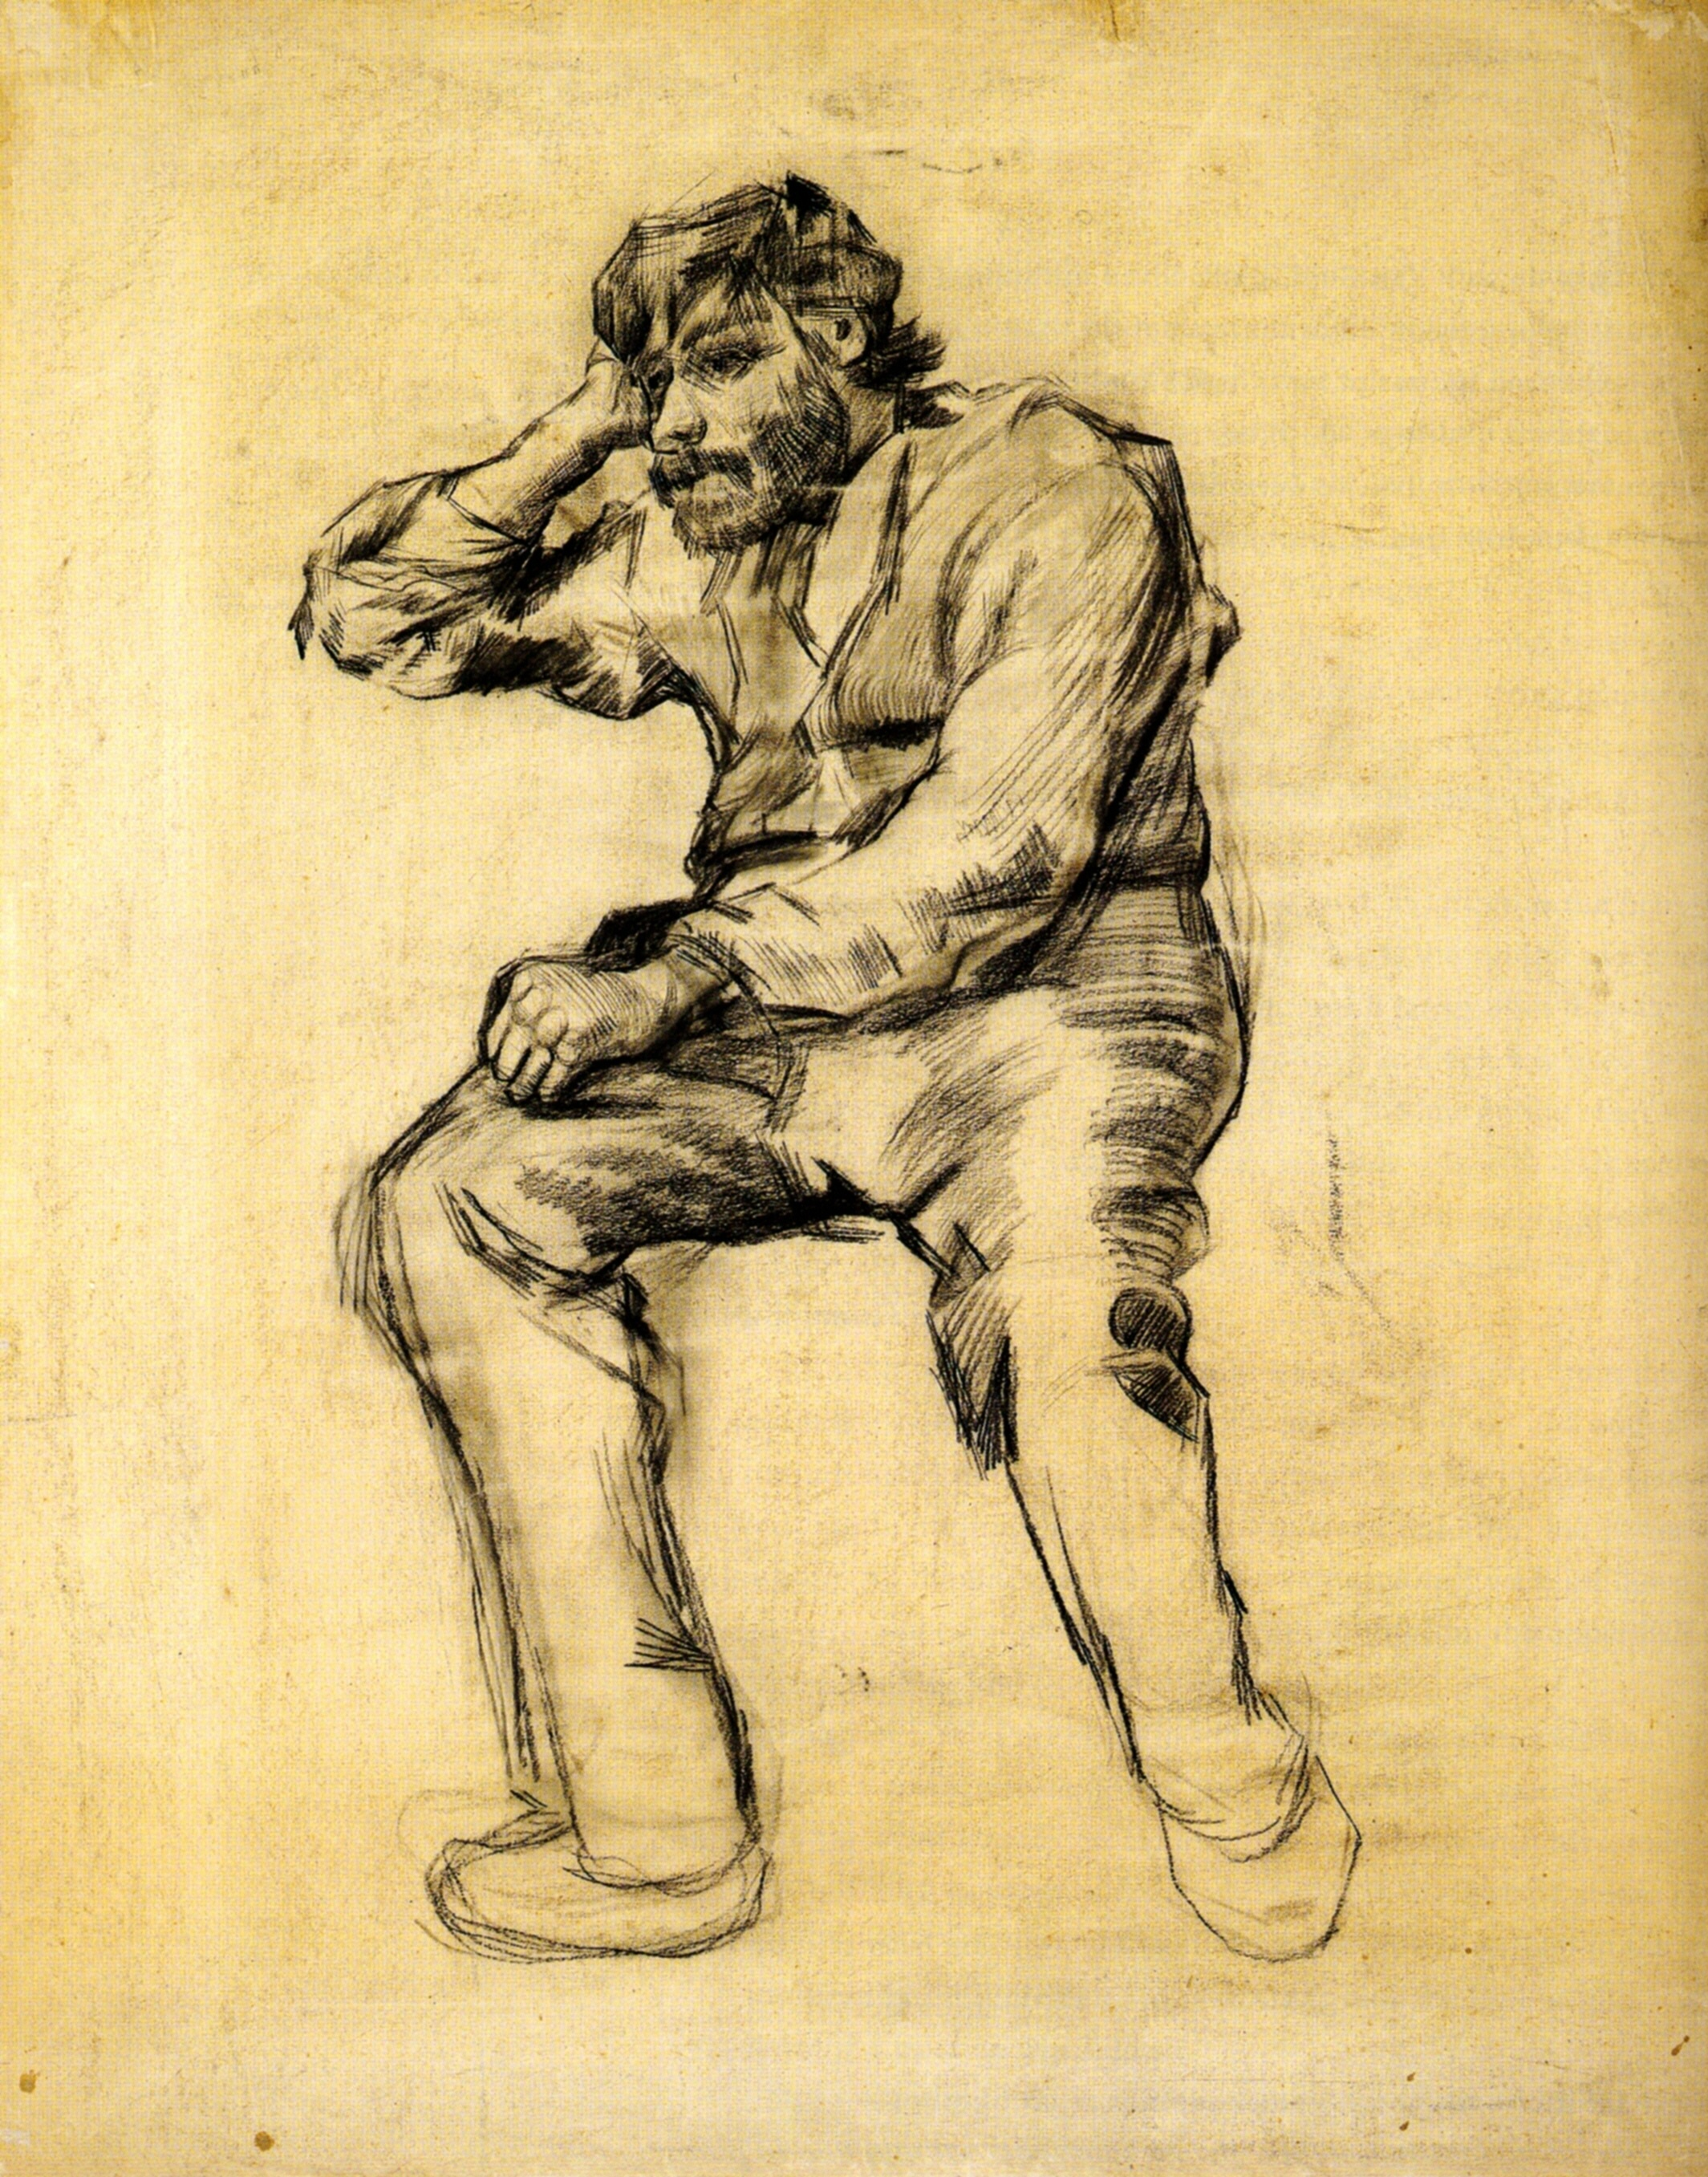
\includegraphics[height=.5\textwidth]{image/vincent-van-gogh_seated-man-with-a-beard-1886-1}
	
	\caption{2 different Van Gogh's artoworks}
	\label{fig:vangogh}
	
\end{figure}

\section{Conclusions and future works}\label{conclusions}
In this essay we present the methods and approaches we have exploited to deal with artist identification. Once again we mark that it's a complex task, without many previous works. 
In our work we were able to reach a top-1 final accuracy of 82\% using ResNeXt with transfer learning, pre-trained on ImageNet, outperforming traditional feature-based approaches by a significant margin, claiming that learning features exploiting the latest CNNs is more performing than hand-crafting them. With the aim to improve our work we think that a larger dataset, both in number of paintings and artists, would allow a significantly increment in accuracy, particularly in training from scratch. 

In future work, we would like to deal with a task that could be considered related to this, namely the recognition of forgeries in art. Our belief is that the representation of style and content learned by our networks would be a good starting point to create a system able to assign a value of authenticity to a painting, because we think that, though is possible to replicate precisely an artifact, the style of an artist is somehow unique and possibly captured by a CNN.

%%% Comment out this section when you \bibliography{references} is enabled.
\begin{thebibliography}{1}
	
	\bibitem{hong2017}
	Yiyu Hong, Jongweon Kim, \newblock  Art Painting Identification using Convolutional Neural Network, \newblock International Journal of Applied Engineering Research, \newblock 2017
	
	\bibitem{Saleh2015}
	B. Saleh and A. M. Elgammal.\newblock  Large-scale classification
	of fine-art paintings: Learning the right metric on the right
	feature. \newblock CoRR, abs/1505.00855, 2015.
	\bibitem{Bar2014}
	W. L. Bar Y., Levy N. Classification of artistic styles using binarized features derived from a deep neural network.
	ECCV 2014.
	
	\bibitem{mensink2014}
	T. Mensink and J. van Gemert. \newblock The rijksmuseum challenge:
	Museum-centered visual recognition. \newblock 2014
	
	
	\bibitem{ArtistIdCNN406}
	Nitin Viswanathan, Standford University,
	\newblock Artist Identification with Convolutional Neural Networks, \newblock 2017
	
	\bibitem{ArtGANDataset}
	\textbf{Dataset:}
	\url{https://github.com/cs-chan/ArtGAN/tree/master/WikiArt Dataset}
	
	\bibitem{Lij2012}
	E. H. J. Li, L. Yao and J. Z. Wang. \newblock Rhythmic brushstrokes
	distinguish van gogh from his contemporaries: Findings via
	automated brushstroke extractions. IEEE Trans. Pattern
	Anal. Mach. Intell, \newblock 2012.
		
	\bibitem{lombardi05}
	T. E. Lombardi. \newblock The classification of style in fine-art painting. ETD Collection for Pace University, \newblock 2005.
	
	\bibitem{jou2011}
	J. Jou and S. Agrawal. Artist identification for renaissance
	paintings, 2011.
	
	\bibitem{razavian2014}
	A. H. S. J. C. S. Sharif Razavian, A. Cnn features off-theshelf: An astounding baseline for recognition, 2014.
	
	\bibitem{resnet}
	Kaiming He, Xiangyu Zhang, Shaoqing Ren, Jian Sun. Microsoft Research. 
	Deep Residual Learning for Image Recognition. 2015
	
	\bibitem{resneXt}
	Saining Xie, Ross Girshick, Piotr Dollar, Zhuowen Tu, Kaiming He. UC San Diego - Facebook AI Research. Aggregated Residual Transformations for Deep Neural Networks, 2017.
	
	\bibitem{googlenet}
	Christian Szegedy, Wei Liu, Yangqing Jia, Pierre Sermanet, Scott Reed, Dragomir Anguelov, Dumitru Erhan, Vincent Vanhoucke, Andrew Rabinovich. Going Deeper with Convolutions. 2014
	
	\bibitem{alexnet}
	Alex Krizhevsky, Ilya Sutskever, Geoffrey E. Hinton. ImageNet Classification with Deep Convolutional
	Neural Networks. 2012

	\bibitem{pytorchguide}
	Sasank Chilamkurthy. \url{https://pytorch.org/tutorials/beginner/transfer_learning_tutorial.html}
	
	\bibitem{dropout}
	G. E. Hinton, N. Srivastava, A. Krizhevsky, I. Sutskever and R. R. Salakhutdinov.
	Improving neural networks by preventing co-adaptation of feature detectors. 2012
	
	\bibitem{imagenet}
	ImageNet: \url{http://www.image-net.org/}
	
	\bibitem{pytorch}
	Pytorch: \url{https://pytorch.org/}
	
	\bibitem{vmconfig}
	Virtual Machine pre-settings: \url{https://console.cloud.google.com/marketplace/details/click-to-deploy-images/deeplearning}
	
	\bibitem{gcloud}
	Google Cloud Platform: \url{https://cloud.google.com/}

	
\end{thebibliography}


\end{document}